% Пример заготовки для презентации с использованием класса Beamer LaTeX.
% Версия от 09 ноября 2018 года.
\documentclass[12pt,a4paper,mathserif]{beamer}
\usepackage[utf8x]{inputenc}
\usepackage{ucs}
\usepackage[T2A]{fontenc}
\usepackage[english,russian]{babel}
\usepackage{amsmath}
\usepackage{amsfonts}
\usepackage{amssymb}
\usepackage{mathtext}
\usepackage{graphicx}
\usepackage{enumerate}
\usepackage{multirow}
\usepackage{ragged2e}
% Пакет для оформления исходного кода
\usepackage{minted}
\usepackage{adjustbox}
\justifying
\renewcommand{\raggedright}{\leftskip=0pt \rightskip=0pt plus 0cm}
\setbeamertemplate{caption}[numbered]

\usetheme {Madrid}
\usecolortheme [RGB={85, 107, 47}]{structure} %Dark Olive Green

\author[Лаптев А.В.]{{Cтудент 595 группы: Лаптев А.~В.}\\
{Научный руководитель: Шмаков И.~А.}}
\title{Проблема дребезга кнопок в устройствах персонального типа}
% \subtitle{Отчет по научно-исследовательской работе}

\begin{document}
\begin{frame}
\maketitle
\end{frame}

\begin{frame}{Актуальность}
    \setlength{\parindent}{0.5cm}
    Различные кнопки и переключатели встречаются в цифровой аппаратуре повсеместно, поэтому проблема дребезга контактов в них зачастую является существенной. Дребезг контактов может стать причиной неправильной работы устройства в следствие неверного распознавания переключения или нажатия или отжатия кнопки, а это в ряде случаев может стать критичным даже для человека.
\end{frame}

\begin{frame}{Устранение эффекта дребезга контактов}
    \setlength{\parindent}{0.5cm}
    Для подавления дребезга контактов в электронных схемах существует два пути:

    \begin{enumerate}
        \item Решение программным путем
        
        \begin{enumerate}
            \item Использование задержек
    
            \item Использование циклического опроса состояния кнопки
        
            \item Использование прерываний по состоянию вывода порта 
        \end{enumerate}
    
        \item Решение аппаратным путем

        \begin{enumerate}
            \item Сглаживающие фильтры
    
            \item RS-триггер
        
            \item Использование одновибратора (ждущего мультивибратора)
        \end{enumerate}
    \end{enumerate}
\end{frame}

\begin{frame}{Программные решения\\Использование задержки}
    \setlength{\parindent}{0.5cm}
    Самым простым способом справиться с проблемой дребезга кнопки является выдерживание паузы. Микроконтроллер останавливается и ждет, пока переходный процесс не завершится. Для этого можно использовать любую встроенную функцию задержки, интегрированную в язык программирования. 10-50 миллисекунд обычно для большинства случаев.
\end{frame}

\begin{frame}{Программные решения\\Использование циклического опроса состояния кнопки}
    \setlength{\parindent}{0.5cm}
    Данный способ представляет собой циклическое считывание состояния кнопки с установленным интервалом считывания (обычно примерно 0,5-5 мс). Эта операция может выполняться как внутри основного цикла программы, так и в процедуре обработки прерываний таймера, которые будут происходить с той же частотой.
\end{frame}

\begin{frame}{Программные решения\\Использование прерываний по состоянию вывода порта}
    \setlength{\parindent}{0.5cm}
    Микроконтроллер запоминает состояние, 0 или 1, для заданного вывода порта. Когда состояние меняется, не важно, из 0 в 1, или из 1 в 0, микроконтроллер генерирует прерывание. В некоторых случаях можно задавать какое изменение (0-1 или 1-0) генерирует прерывание. Дополнительно может потребоваться выполнять чтение порта, для обновления сохраненной информации о состоянии вывода.
    
    При этом прерывания по изменению состояния вывода порта нужно заблокировать на время гашения дребезга контактов. Это исключает влияние дребезга на состояние кнопки в программе.
    
    По истечении заданного времени гашения дребезга снова разрешаются прерывания по изменению состояния вывода порта.
\end{frame}

\begin{frame}{Аппаратные решения\\Сглаживающие фильтры}
    \begin{figure}
        \centering
        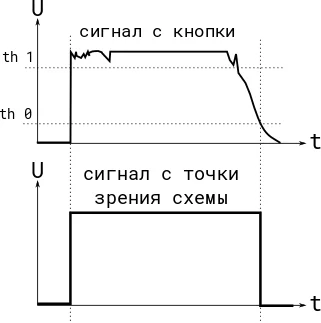
\includegraphics[scale=0.8]{shmidt.png}
        \label{fig:shmidt}
    \end{figure}
\end{frame}

\begin{frame}{Аппаратные решения\\RS-триггер}
    \begin{figure}
        \centering
        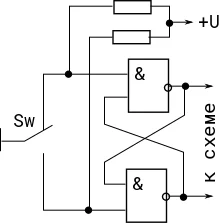
\includegraphics{RS.png}
        \label{fig:rs}
    \end{figure}
\end{frame}

\begin{frame}{Аппаратные решения\\Использование одновибратора (ждущего мультивибратора)}
    \begin{figure}
        \centering
        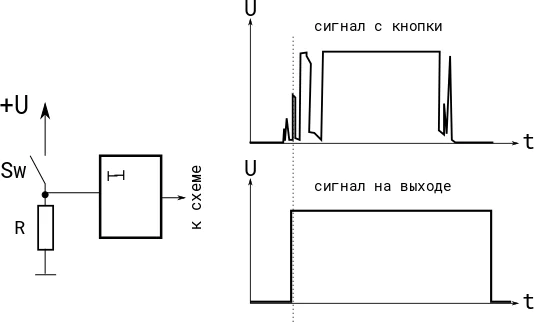
\includegraphics[scale=0.6]{vibrator.png}
        \label{fig:vibrator}
    \end{figure}
\end{frame}

\begin{frame}{Выбор метода для подавления дребезга для проекта}
    \setlength{\parindent}{0.5cm}
    В результате проведенного анализа и практического применения части рассмотренных способов гашения дребезга был выбран программный метод гашения дребезга путем использования прерываний. Поскольку данный способ не требует внесения изменений в схему устройства и является эффективным, поскольку не требует останавливать работу устройства, как это происходит при использовании задержек и программа не будет тратить время на постоянный опрос состояния кнопки, как при использовании циклического опроса.
\end{frame}

\begin{frame}{Алгоритм для подавления дребезга}
    \begin{figure}
        \centering
        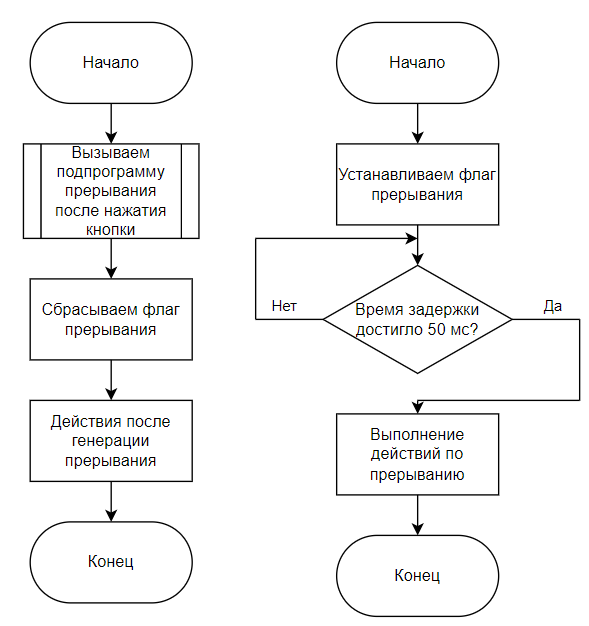
\includegraphics[scale=0.4]{algorithm.png}
        \label{fig:algorithm}
    \end{figure}
\end{frame}

\newlength\someheight
\setlength\someheight{3,5cm}

\begin{frame}[fragile]{Реализация алгоритма с использованием Arduino IDE}
    \begin{adjustbox}{width=\textwidth,height=\someheight,keepaspectratio}
    \begin{minipage}{1\linewidth}
    \begin{minted}{C++} 
volatile boolean chatterFlag = false; 
 
void setup() {
  Serial.begin(9600);
  pinMode(2, INPUT_PULLUP); 
  attachInterrupt(0, chatter, FALLING);
}
 
volatile uint32_t chatter_time;
void chatter() {
  chatterFlag = true;
  // 50 подавляем дребезг кнопки, читаем состояние порта
  if (millis() - chatter_time >= 50 && digitalRead(2))
  {
    chatter_time = millis();
    // Дальнейший код прерывания
  }
}
 
void loop() {
  if (chatterFlag) {
    chatterFlag = false;    
    // Действия после генерации прерывания
  } 
    delay(1000);              
}
    \end{minted}
    \end{minipage}
    \end{adjustbox}
\end{frame}

\begin{frame}{Выводы}
    \setlength{\parindent}{0.5cm}
    Использование данного метода для подавления дребезга позволило полностью избавиться от влияния дребезга контактов на работу устройства на отладочной плате, которая использовалась для тестирования работоспособности генератора персонажа DnD.
\end{frame}

\end{document}
